\documentclass[fr]{../../../eplsummary}
\usepackage[french]{varioref} % \vref and \vpageref
\usepackage{graphicx} % images
\usepackage{float} % images
\usepackage{url}
	\urlstyle{sf}
\usepackage[backgroundcolor=yellow]{todonotes} %% todonotes: \listoftodos & \todo{Some note or other.} & \missingfigure{}

% draw
\usepackage{tikz}
\usetikzlibrary{arrows}
% \usepackage{qtree}    % dessiner des arbres %% => texlive-humanities

\definecolor{codeBlue}{rgb}{0,0,1}
\definecolor{webred}{rgb}{0.5,0,0}
\definecolor{codeGreen}{rgb}{0,0.5,0}
\definecolor{codeGrey}{rgb}{0.6,0.6,0.6}
\definecolor{webdarkblue}{rgb}{0,0,0.4}
\definecolor{webgreen}{rgb}{0,0.3,0}
\definecolor{webblue}{rgb}{0,0,0.8}
\definecolor{orange}{rgb}{0.7,0.1,0.1}

\usepackage{caption}
\renewcommand{\familydefault}{\sfdefault}

\usepackage{listings}		% Pour l'insersion de fichiers de codes sources.
\lstset{
	  language=Java,
	  frame=single,
	  flexiblecolumns=true,
	  numbers=none, % left
	  stepnumber=1,
	  numberstyle=\ttfamily\tiny,
	  keywordstyle=\ttfamily\textcolor{blue},
	  stringstyle=\ttfamily\textcolor{red},
	  commentstyle=\ttfamily\textcolor{green},
	  breaklines=true,
	  extendedchars=true,
	  basicstyle=\ttfamily\scriptsize,
	  showstringspaces=false
	}

\lstdefinelanguage{diff}{
  morecomment=[f][\color{blue}]{@@},     % group identifier
  morecomment=[f][\color{red}]-,         % deleted lines
  morecomment=[f][\color{green}]+,       % added lines
  morecomment=[f][\color{magenta}]{---}, % Diff header lines (must appear after +,-)
  morecomment=[f][\color{magenta}]{+++},
}

\IfFileExists{fourier.sty}{\usepackage{fourier}}{\typeout{! WARNING: Fourier package not included: skip it}}

%%%%%%%%%%%%%%%%%%%%

\title{LINGI2172 - Exams}
\author{Matth, LN, Alex, Ben, Leader, Houtain Nicolas}
\hypertitle{Databases}{8}{INGI}{2172}
{Matthieu Baerts\and Benoît Baufays\and Julien Colmonts\and Alex Vermeylen\and Hélène Verhaeghe}
{Bernard Lambeau}

\section{Lexique}
\begin{itemize}
	\item Variable : C'est une représentation à un temps t de la fonction. La ``table''
	    représente plutôt la valeur de variable.

	    Represent a predicate.
	\item[Notes:] Une table $\neq$ relation puisque la relation est indépendante
	    de l'ordre des rows/columns.

    \item Relation : Fonction qui lie les attributs entre eux.
    \item Attribut : Un champ de la variable
    \item Cardinalité :  Nombre de n-tuple
    \item N-Tuple : une ligne, un ensemble d'attribute value
    \item Tuple : ensemble des lignes
    \item Orthogonalité : %TODO
\end{itemize}


\section{DBMS}

\begin{figure}
    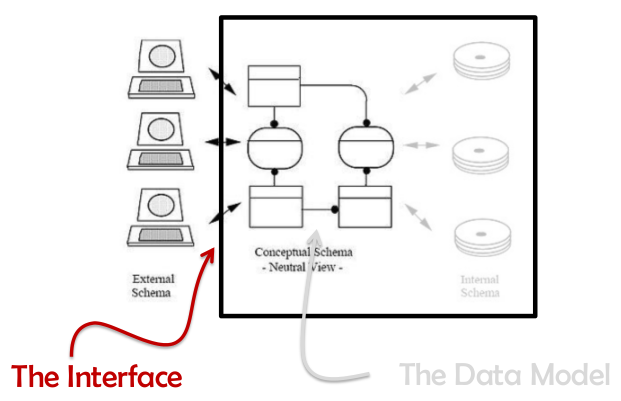
\includegraphics[width=10cm]{img/dbms.png}
    \caption{Database design}
\end{figure}

\begin{description}
    \item[DML] : Data Manipulation Language (manipulate data)
    \item[DDL] : Data Definition Language (manipulate schema, metadata)
\end{description}

\section{Predicate logique}

Une proposition est composé de différent paramètre (ex: $x \leq y$).
P(x), a predicate, is called a membership
predicate for the set consisting of all such objects a.

\begin{itemize}
    \item[Definition]
    \item Intension : its meaning
    \item Extension : all the instantiations that are ``true''
    \item Substitution : replace a paramerter by a \textit{designator}
    \item Instantiation : substitution of all the parameter

    \item[Operator]
    \item Conjunction, disjunction , negation, implication, only if, equivalence

    \item[Quatifiers]
    \item Existential, universal

    \item[Sets]
    \item $\in$, $\subseteq$, $\supseteq$, $\subset$, $\supset$, equality
    \item Join, disjointness, union, intersection, complement, difference
\end{itemize}

\subsection{Tutorial D}

\begin{table}
    \centering
    \begin{tabular}{|l|l|}
        \hline
        \textbf{Logic} & \textbf{Tutorial D} \\
        \hline
        AND & JOIN \\
        & WHERE (restriction) \\
        & EXTEND (extension) \\
        & SUMMARIZE \\
        \hline
        EXISTS & EXISTS (projection) \\
        \hline
        OR & UNION \\
        \hline
        (AND) NOT & MINUS (difference) \\
        & NOT MATCHING (semi-difference) \\
        \hline
        & RENAME \\
        \hline
    \end{tabular}
    \caption{Link Logic operate and Tutorial D}
\end{table}

\subsubsection{JOIN}

Let $s = r_1 JOIN r_2$.
$\to$ Commutative and associative.


\paragraph{Special case :}
\begin{itemize}
    \item R JOIN R = \textbf{R}
    \item If all attributes are common to both operand = \textbf{Intersection}
    \item If no attribute are common to both operand = \textbf{Cartesian product}
\end{itemize}

\subsubsection{EXISTS}
Let $s = r \{A_1, \cdots, A_n\} = r\{ ALL BUT \quad B_1, \cdots, B_m\}$.

\paragraph{The heading of s} = the subset of the heading of r given by $\{A_1, \cdots, A_n\}$.

\paragraph{The body of s} = each tuple that can be formed
from a tuple of r by removing from it the attributes named $\{B_1, \cdots, B_m\}$.

\paragraph{Special case :}
\begin{itemize}
    \item $R \{ ALL BUT \}$ = \textbf{R}
    \item $R \{ \}$ = \textbf{A relation with no attributes at all}
\end{itemize}


\subsubsection{WHERE}
Let $s = R WHERE C$

\paragraph{Special case :}
\begin{itemize}
    \item $R WHERE TRUE$ = \textbf{R}
    \item $R WHERE FALSE$ = \textbf{A empty relation with heading of R}
\end{itemize}

\subsubsection{ TODO }

TODO slide 4b

\subsection{PostgreSQL}

TODO


\section{Constraint}

Constraints express the integrity rules for a database.
They enforcement of constraints by the DBMS ensures that the
database is at all times in a consistent state.

\subsection{KEY constraints}

The key of a relation must be uniqueness. 
A relvar can have several keys : the nominate on is called ``primary key'' and the
other ``alternate keys''.

\subsection{Foreign key}

There is a \textbf{inclusion dependency} because the relation which
contains a foreign key (SECOND) must be included into the relation which
contains the key (FIRST) : $$ FIRST { StudentId } \supseteq SECOND {
StudentId}$$

\paragraph{Superkey} is a combination of columns that uniquely identifies
any row within a function. A superkey become a key when he is reduced to
the minimum number of columns.

\paragraph{Generalisation of inclusion dependency}
$$ IS_EMPTY( SECOND NOT MATCHING FIRST )$$

\paragraph{Multiple assignement} is used when we need to update several
variable on the same time to respect some constraint.



\subsection{Implicit constraint}

A single relvars (which describe ``A'' like : ID\#, Name, Field1,
Field2) have an implicit constraint to the effect that every ``A'' has a
ID, a Name, a Field1 and a Field2\ldots

To avoid this implicit constaint, we need to decomposed the design in
different table link by the a foreign key (ID\#).

\paragraph{ }
The single relvar design is preferred so long as the constraint implied
by it truly reflects the real world!

\section{Normal Form}

\subsection{Fonctional dependency (FD)}\label{fd}

Soit une relation $R$, un set d'attributs (\textbf{determinant}) et
détermine un set (\textbf{dependant set}) $\forall (x \rightarrow y)$
si et seulement si chaque valeur de $x$ est associée à un élément de
$y$. Note that a FD denotes a function.

For example, in the relation $a+b=c$ we have $\{a,b\} \rightarrow \{c\}$.

\paragraph{Theorem about FD: }
\begin{itemize}
    \item Left augmentation : if A' is a superset of A, then A' $\to$ B 
    \item Right reduction : if B' is a subset of B, then A $\to$ B' 
    \item Transivity : if A $\to$ B and B $\to$ C, then A $\to$ C 
    \item General : if A $\to$ B and C $\to$ D, then A $\cup ( C - B) \to B \cup D$
    \item[]
    \item Left-irreducibility : if A $\to$ B and there is no proper subset A' such
        that A' $\to$ B, then A $\to$ B is \textbf{left-irreducible} and B is said
        \textit{fully dependent} on A.
    \item[]
    \item A is a superkey of r if A $\to$ B and A $\cup$ B constitutes the entire
        heading of r
    \item A is a key of r if A $\to$ B is left-irreducible and A $\cup$ B constitutes the entire
        heading of r
\end{itemize}

\subsection{Join dependency}\label{jd}

Une relation est sujette à une join dependency si elle peut être
recréée en joignant plusieurs tables ayant chacune un sous ensemble
des attributs de la relation.

On parle de \textit{join dependency triviale} si une des tables du join
à tous les attributs de la relation initiale: bref que l'on ne peut
plus faire de join dependency (voir exemple en section \vref{6NF}).

\subsection{1 NF}

A relation is in 1NF if attribute domains include only
atomic (simple, indivisible) values and each tuple
attribute value is a single value from the domain.

% http://www.tablesgenerator.com/#
% http://truben.no/latex/table/
\begin{table}[H]
\begin{tabular}{|c|c|c|}
\hline
A$_1$ & A$_2$ & A$_3$ \\ \hline
      &       &       \\ \hline
      &       &       \\ \hline
\end{tabular}
\hfill
\begin{tabular}{|c|c|c|}
\hline
A$_1$ & A$_2$ & A$_3$ \\ \hline
      &   \rule{0pt}{3ex} \begin{tabular}{|c|c|}\hline & \\ \hline \end{tabular}    &       \\ \hline
      &   \rule{0pt}{3ex} \begin{tabular}{|c|c|}\hline & \\ \hline \end{tabular}    &       \\ \hline
\end{tabular}
\hfill
\begin{tabular}{|c|c|c|}
\hline
A$_1$ & A$_2$ & A$_3$ \\ \hline
      &   \rule{0pt}{5ex} \begin{tabular}{|c|}\hline \\\hline \\ \hline \end{tabular}    &       \\ \hline
      &   \rule{0pt}{5ex} \begin{tabular}{|c|}\hline \\\hline \\ \hline \end{tabular}    &       \\ \hline
\end{tabular}
\end{table}

The first is good, but in the second there is no atomic value (there is a tuple)
and in the third we have no simple value.

\subsection{3 NF}
Source: Wikipédia.\\
Doit premièrement être 2 NF: tout attribut \textit{non-prime} (donc pas dans une clé) doit dépendre d'une clé entière (pas juste certains attributs).

Ensuite, tout \textit{non-prime} ne peut être transitivement dépendant ($A \rightarrow B, B \rightarrow C$: $C$ est transitivement dépendant de $A$) de toutes super keys de R.\\

On peut également définir par cette définition : Pour toute dépendance fonctionnelle ($X \rightarrow A$), il doit y avoir au moins une de ces 3 conditions qui soit correcte:
\begin{itemize}
	\item $X$ contient $A$ ($A\subseteq X$)  (FD triviale, voir section \vref{fd})
    \item $X$ est une superkey (voir section \vref{key})
    \item chaque élément de $A \backslash \{X\}$ est \textit{prime} (est contenu dans une clé)
\end{itemize}

\subsection{BCNF}
Pour toutes dépendances fonctionnelles (voir section \vref{fd}) $X \rightarrow A$, il doit y avoir au-moins une de ces 2 conditions respectées:
\begin{itemize}
	\item $X$ contient $A$ ($A\subseteq X$)  (FD triviale, voir section \vref{fd})
    \item $X$ est une superkey (voir section \vref{key})
\end{itemize}

%TODO advantages of BCNF 

\subsection{5 NF}
Une relation est 5NF si toutes \textit{join dependencies} (voir section \vref{jd}) non-triviales est implicite par les candidate keys (= super key quand il n'y a pas encore de clé primaire): \textit{join dependencies} à $\{A, B, ..., Z\}$ est implicite par les candidates keys si et seulement si chaque $A, B, ..., Z$ est superkey.

\subsection{6 NF}\label{6NF}
Une relation est 6NF si elle ne satisfait aucune \textit{join dependency} (autre que les triviales donc).\\

\begin{table}[H]
\begin{center}
\begin{tabular}{|l|l|l|l|l|l|l|l|}
\cline{1-2} \cline{4-5} \cline{7-8}
\textbf{ID} & \textbf{FName} & \textbf{} & \textbf{ID} & \textbf{LName} & \textbf{} & \textbf{ID} & \textbf{Status} \\ \cline{1-2} \cline{4-5} \cline{7-8}
1           & Alex           &           & 1           & Vermeylen      &           & 1           & Sleeping        \\ \cline{1-2} \cline{4-5} \cline{7-8}
2           & LN             &           & 2           & Verhaeghe      &           & 2           & Watching TV     \\ \cline{1-2} \cline{4-5} \cline{7-8}
\end{tabular}
\caption{Exemple de 6NF}
\end{center}
\end{table}
On ne peut plus faire de join dependency mais du coup, c'est dangereux: si on ajoute une nouvelle entrée dans la première table, il faut ajouter des contraintes pour être sûr d'ajouter aussi dans les autres tables si c'est nécessaire.

\subsection{Heath's theorem}
%TODO


\section{View, Rules \& Triggers}

\subsection{View}

View are relation variables (capture predicate extension, should be updatable,
have constraints and have keys).

But, unlike ``BASE'', they should be kept hidden to end-users.


\subsubsection{View updating}


\subsection{Rules \& Triggers}


Ce sont tous les deux des objets de base de données mais les
triggers sont attachés à une table et uniquement déclanché après
qu'un \texttt{INSERT}, un \texttt{UPDATE} ou un \texttt{DELETE} ait
été utilisé. Donc en gros, c'est pour exécuter une requête
automatiquement lorsqu'un tel événement a lieu. Attention, ceci peut
être fait avant ou après (à spécifier à la création du trigger),
donc pas forcément à postériori mais en tous cas, le trigger ne
modifie pas l'AST! (et il ne peut donc pas annuler des opérations, etc.
alors qu'avec un \textit{rule}, on peut avec \texttt{INSTEAD NOTHING})\\

Alex (en parlant de Triggers vs. \textbf{Rules}): Je dirais plus que la
différence principale c'est que le trigger ne se déclenche réellement
qu'après que l'insert (ou autre opération) ait été achevé ; alors
que la rule elle, modifie l'AST (arbre représentant l'execution plan
pour une query) et donc, le code produit pour faire la query est
différent et tient compte de cette rule.

De ce fait, la rule est plus efficace que le trigger. Si on fait 100
insert, on exécute 100 fois le trigger ; alors que si on modifie
l'arbre, on ne doit construire qu'une seule fois cet arbre. Le travail
est donc le même pour une ou 100 query(ies).

En outre, la rule peut être utilisé avec une view, alors que le
trigger, ne peut pas.

\section{ACID}
Toutes les transactions doivent être ACID pour être relationnelles. ACID:
\begin{itemize}
	\item Atomic: toute la transaction se fait en une fois: si ça plante, ça revient à l'état d'avant
    \item Concistant: toutes les contraintes sont vérifiées
    \item Isolated: il vaut pouvoir gérer les concurrences
    \item Durability: une fois que la transaction est fini, l'état est changé et il est durable...
\end{itemize}

\section{Other Material}
\subsection{S3}
Pour l'union, elle est bien commutative (on s'en fout du résultat et du truc bizarre sur SQL, la question c'est "est-ce que l'union est commutative").

\subsection{S4}
Voir mémoire.

\subsection{S5}
On peut utiliser un \texttt{EXTEND}:
\begin{lstlisting}
EXTEND NOM_DE_LA_TABLE : {NOM_NOUVELLE_COLONNE}
EXTEND SUPPLIERS : {TOTAL := COUNT(SUPPLIERS), TOTAL2 := COUNT(PARTS)}
\end{lstlisting}

\subsection{S9}
EER: Enhanced Entity-Relationship Model, a high-level conceptual data model extended from the Entity-Relationship Model. Source: Kikipedia (\url{https://en.wikipedia.org/wiki/Enhanced_Entity-Relationship_Model}). ER est en top-down.

%\begin{center}
%	\includegraphics[width=.75\textwidth]{pub2.png} % merci Ben :)
%\end{center}

\subsection{A bottom-up design method}
 The bottom-up approach begins with the specific details and moves up to the general.  To begin a bottom-up design, the system analyst will inspect all the interfaces that the system has, checking reports, screens, and forms.  The analyst will work backwards through the system to determine what data should be  stored in the database.\\

To understand the differences between these approaches, let's consider some jobs that are bottom-up in nature.  In statistical analysis, analysts are taught to take a sample from a small population and then infer the results to the overall population.  Physicians are also trained in the bottom-up approach.  Doctors examine specific symptoms and then infer the general disease that causes the symptoms.\\

\subsection{Database designs}
\subsubsection{Le meilleur}
Ça dépend toujours du design...

\subsubsection{With respect to real-world requirements}
\todo{Julien}

\subsubsection{Underlying objectives}
Les NF aide à faire ça
\begin{itemize}
  \item Avoid Redundancy: Si on a du 5NF, on évite la redondance car
  \item Update Anomalies: Pas en 6NF
  \item Achieve Simplicity: En 6NF
  \item Orthogonality: (plus c'est séparé, plus c'est orthogonale), ex: 6NF (peut-être même trop)
\end{itemize}

\subsubsection{Typical exam question}
\todo{TODO: Julien}
L'oracle sert à prédire le reste.\\
Décomposer R en R$_1$ ... R$_n$ en BCNF: voir définition de BCNF, c'est le match de la Suisse en ce moment... (\textit{Il faut que la clé implique}). \textbf{Il y a un algo dans les slides}.\\
Tutorial D: voir match Suisse -- Equateur.

\section{Exam}


\subsection{Expliquer pourquoi l'implémentation des views dans PostGreSQL brise la règle de Logical Dependencies}


\subsection{Donner les avantages et inconvénients des databases JSON suivant certains requirements}
\begin{itemize}
	\item Communiquer directement avec la DB).
    \item JSON comme une base de données (like NoSQL). Mais ce n'est pas relationnel -> c'est la merde de mettre ca dans un type de base de données relationnel (pas 1NF)
    \item compare c'est la merde
    \item si tu chopes un JSON pour ta DB, tu peux le save
    \item si TYPE en REL, on peut ajouter des opérateurs
\end{itemize}

\subsection{Atomicity of ACID}
La transaction est vue comme une seule transaction, même si elle est constituée de plein de petites transactions. Donc, l'atomicité consiste à voir une trnsaction comme si c'était une seule opération. De ce fait, soit la transaction réussi et est effectuée, soit la transaction plante et donc, rien n'est fait (comme si on avait pas fait de tansaction).

Pour assurer l'atomicité (quand une transaction plante) :
\begin{itemize}
  \item Undo log : reverse action déjà faites
  \item Redo log : je retente les actions déjà faites
  \item mélange de undo/redo : je fais une soupe
  \item rollback/checkpoint : plus nouvelles transactions.  Quand fini, checkpoint (sauve DB) et je reviens la si c'est la merde
  \item Backup DB : j'utilise mon backup
\end{itemize}

\subsection{Consistant of ACID}
Les contraintes doivent toujours être vérifiées.\\
Commit se fait que si toutes les contraintes sont vérifiées.\\
Rollback on revient au dernier état consistant.\\
\subsection{Isolation of ACID}
Toutes les transactions sont serializable ().\\
Implémenté avec des LOCK.  Read Only et Write Only.  Toujours dans le même ordre sont pris les lock.\\


\subsection{Les DB sont basées sur la théorie des ensembles.  Montrez le dans l'algèbre relationnelle}
Les types sont des ensembles de valeurs.\\
\texttt{NOT MATCHING} (disjonction), \texttt{MATCHING} (intersection), \texttt{WHERE} (appartenance)

\subsection{Pourquoi certaines versions de SQL ne permette pas d'updater les views ?}
Quand on update la view, on update pas les tables qu'elle utilise. Il faut créer une rule qui update les tables. Mais pas dispo dans toutes les versions.


\subsection{Index dans Postgresql}
Source: \url{https://dev.mysql.com/doc/refman/5.0/fr/mysql-indexes.html}.

Tous les index de MySQL (\texttt{PRIMARY}, \texttt{UNIQUE} et \texttt{INDEX}) sont stockés sous la forme de \texttt{B-tree}. Les chaînes sont automatiquement préfixée et leurs espaces terminaux sont supprimés.

En PostgreSQL, B-tree, R-tree, Hash ou GiST.

\subsection{Expliquer l'indépendance des données (logique et physique)}
Dépendance physique : Peut importante le support, ca doit toujours être la même représentation.\\
Dépendance logique : Dépendant dans l'idée mais pas la même entre la DB et le programme\\

\subsection{En quoi l'architecture ANSI-SPARC en est liée avec le data model}
Il s’agit de l’architecture fondamentale sur laquelle reposent les SGBD modernes, elle fut proposée en 1965 par Charles Bachman qui reçut le prix Turing pour ses travaux. L’architecture Ansi-Sparc est divisée en trois niveaux, celui du schéma interne (SI), celui du schéma conceptuel (SC) et celui des schémas externes (SE).\\
La première innovation de l’architecture Ansi-Sparc est la distinction claire entre la représentation interne des données au niveau physique (structure de données) et la représentation logique de celles-ci. Une base de données est définie et manipulée via le niveau conceptuel (SC) sans avoir à se soucier des détails de l’implémentation physique (SI). Par exemple, il est possible de définir un index sur un ensemble de données, mais comment celui-ci est réalisé au niveau physique n’a pas besoin d’être spécifié. Sur le même principe, lors d’une requête, l’usager n’a pas besoin d’indiquer comment utiliser l’index pour maximiser l’efficacité de la recherche.
La deuxième grande innovation de ce modèle est la possibilité de créer des schémas externes qui sont en fait des portions de la base de données (sous-bases virtuelles) destinées à différents usagers. Un usager particulier ne peut manipuler que les données appartenant à son propre schéma externe. De nos jours, le terme schéma externe est remplacé par celui de « vue ».\\
\subsection{Définir une relation et donner le lien avec le first order logique}
une relation c'est un ensemble de tuple qui vérifie une propriété.\\
Le first order les prédicats qui peuvent être instanciées en fonction des variables (soit vrai soit fausse) et au final la propriété peut être un prédicat.  Les tuples pouvant être acceptés sont ceux qui vérifient un prédicat.\\
Closed world assumption : l'entièreté des tuples peuvent être mis dans la relation.  On suppose que la relation a tous les tuples.
\subsection{BCNF}
Table donnée.  Créée une nouvelle relation.  Pourquoi pas BCNF ?  FD uniquement trivial ou X super Key.  Or, ici cours est toujours=C1.  FD Point vers cours et point n'est pas superkey, donc merdoum.
\subsection{Requete et le query plan donné.  Que fait l'optimizer ?}
Associativité : restriction sur chaque avant de join.\\
Mettre un clustering index et un index primaire sur les quantités.

\subsection{Question Vincent}
\subsubsection{Requête}
1 question avec une requete à faire, et dire comment j'aurais pu faire pour la mettre comme contrainte dans ma DB en tuto D. Et aussi en SQL. La question c'etait genre, dans l'exemple suppliers, shipments, parts s'assurer qu'un fournisseur localiser à Paris ne puisse pas founir plus de 3 parts différentes. je fais le summarize et je dis where countPID > 3 et je dis que ca dois etre = TABLE\_DEE. Pour sql j'ai récris la requete et j'ai dis qu'il faudrait mettre dans un trigers qu'il verifie la contrainte a chaque fois qu'un shipment est insérer $\Rightarrow$ faut une rules plutôt!

\subsubsection{closed world assumption}
"closed world assumption" in database field et expliquer en quoi c'etait relié à la théorie des prédicats dans la logique du premier ordre. $\Rightarrow$ Closed pour 'fermé'. Venant de Kikipedia:

La notion d'hypothèse de monde clos est utilisée en particulier en Prolog, elle s'oppose à l'hypothèse de monde ouvert (voir aussi l'article Logique argumentative) et concerne la question du vrai et du faux.

Elle signifie qu'un fait est considéré comme faux si, en un temps fini, on échoue à montrer qu'il est vrai, ce qui revient à dire que tout ce qui est vrai doit être connu (inclus dans la base de données des faits) ou démontrable en temps fini, il n’y a pas de monde extérieur qui pourrait contenir des éléments de preuve inconnus du programme. Pour les faits vrais, l'hypothèse de monde clos ne dit rien de particulier.

Avec l'hypothèse de monde clos, l'univers des faits se partage entre les faits 'vrai' prouvables en temps fini et tout le reste, assimilé au faux (pour ce qui est accessible en temps fini). Outre la question de la terminaison, cela impose une utilisation du 'faux' avec précaution. Autant le 'vrai' est fort (il ne dépend que de la base de faits et de règles initiale acceptée et du mode d'inférence adopté), autant le 'faux' dépend de l'exhaustivité de la base de faits et de la complétude de la base de règle (2 notions délicates à obtenir).\\

Relation avec la DB: This 1:1 correspondence reflects the Closed-World Assumption:
\begin{itemize}
	\item A tuple representing a true instantiation is in the relation.
	\item A tuple representing a false one is out.
\end{itemize}
(and vice-versa, with respect to the database vs. the world)
The Closed-World Assumption underpins the operators we are
about to meet.
i.e. Algebra operators do not create new facts out of nowhere

\subsubsection{ACID}
il me demandait d'expliquer ce qu'etais l'atomicité d'une transaction et comment on pouvait implementer ca

j'ai dû définir relation et faire le lien avec la logique du premier ordre

\subsection{Question Ricetti}

ACID

une question de porc sur un algo rela que jai pas su faire mais le prof ma dit que cetaitt la plus dure de tte les question
KeRANK r { a1 , a2 , a3 ,... ak }

\subsection{INSERT/DELETE/UPDATE sont des shorthands pour une assignation de relvar}
Shorthands pour raccourcis je suppose...
\begin{itemize}
	\item INSERT, for adding tuples to a relvar
	\item UPDATE, for updating existing tuples in a relvar
	\item DELETE, for removing tuples from a relvar
\end{itemize}

\subsection{Comment optimiser les DB qui tiennent entièrement en RAM}
Que mettre dedans? Si on doit choisir, d'abord l'index. Si c'est tout, faut-il optimiser le temps d'accès ou la place? Et donc en gros, répondre à: comment arranger les info?\\
Vu que c'est du random access memory, on s'en fout où c'est en mémoire (toujours le même temps d'accès, peu importe où on doit aller).
\begin{itemize}
	\item Si on doit minimiser la place, vaut mieux éviter plein de références et avoir tout en un bloc (si on sait que la suite est juste après, pas besoin d'utiliser de la mémoire pour dire que le bloc suivant est à l'adresse X, ça occupe de la place...  $\Rightarrow$ donc plus dans l'idée d'utiliser surtout un primary index (voir multi-level pour profiter des B-Trees) et donc un \textit{sparse} index pour avoir une index que sur qqs search values.
    \item d'un autre côté si on veut optimiser le temps d'accès, c'est intéressant d'avoir plein de jumps pour éviter de tout lire et directement avoir ce que l'on veut surtout que le coût des jumps en terme de temps est (quasi) nul $\Rightarrow$ secondary Index et donc avec un index \textit{dense}: une entrée dans l'index pour chaque valeur recherchée.
\end{itemize}
Mais ça m'a l'air faible comme explication...\\
Pour moi l'idée est de profiter du temps d'accès ultra rapide peu importe où se situe l'info. Si on a plein de jumps, sur un disque dur, c'est lent.\\
Note: en RAM, s'il n'y a plus de courant... tout est parti!

\end{document}
